\subsection{Drivhus styring}

I kundens drivhus skal der dyrkes tomater og agurker som har fordel af en relativ luftfugtighed på 70\% - 80\%.
Da dette drivhus ikke er opvarmet, så bliver tomatplanterne udplantet omkring den 1. maj og agurk planterne i slutningen af maj.
Temperaturen i drivhus bør i dagstimerne være mellem 20$^\circ$C - 30$^\circ$C, og helst ikke meget over, da planterne ikke kan holde til varmen.

\subsubsection{Luftfugtighed}
Luftfugtighed fortæller hvor mange gram vand der er i en m$^3$ luft ved en given temperatur.
Hvis vi kigger på figure \ref{fig:luft_vanddamp}, så kan der ses at mængden af vand som luften kan optage er en konstant, men er afhængelige af temperaturen.
Det kan også ses at det ikke er en linære afhængelig af temperaturen.
Så tit ville man bruge relativ luftfugtighed (angivet som \%RF eller \%RH), som angiver luftfugtighed som en er procentsats. 
Da enheden bliver temperatur uafhængeligt og siger om hvor meget vand der i forhold til luften.

%Tomat i drivhus uden varme er fra omkring 1. maj
%Agurk i drivhus uden varme og som små planter i slutningen af maj til juni.

%Begge planter kan ikke klar temperature over 30 grader celcius.

%Luftfugtighed ønskes til at være omkring.

%Reduktion af Luftfugtighed kan ske via ventilation. \url{http://pure.au.dk/portal/files/42028244/743458.pdf}
%Luftfugtighed agurk: 2 g kg$^{-1}$ 
%Luftfugtighed tomat: 3 g kg$^{-1}$ 
%80 \% RH

%\url{https://www.havenyt.dk/spoergsmaal/drivhuset/12188.html}
%Tomater: 20 grader om dagen
%Agurk: 26 - 28 grader om dagen
%\url{https://voresvilla.dk/haven/drivhus-orangeri/undga-sygdomme-drivhuset/}
%Op til 4 liter vand om dagen.
%\url{http://old.gyproc.dk/files/Gyproc/Library/Handbook/DK/HB9%20-%204.5.2%20-%20Fugt%20i%20luft.pdf}
%\url{http://www.vitavia.dk/filarkiv/pdf/Vitavia_broc_2017_DK_low.pdf}

\begin{figure}[!h]
    \begin{center}
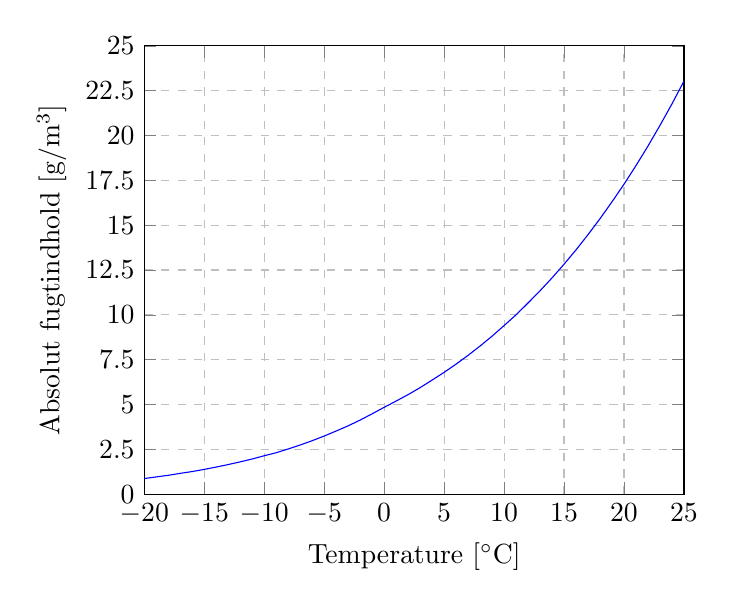
\begin{tikzpicture}
\begin{axis}[
    %title={Luft mættet med vanddamp},
    xlabel={Temperature [$^{\circ}$C]},
    ylabel={Absolut fugtindhold [g/m$^3$]},
    xmin=-20, xmax=25,
    ymin=0, ymax=25,
    xtick={-20, -15, -10, -5, 0, 5, 10, 15, 20, 25},
    ytick={0.0, 2.5, 5.0, 7.5, 10.0, 12.5, 15.0, 17.5, 20.0, 22.5, 25.0},
    %legend pos=north west,
    ymajorgrids=true,
    xmajorgrids=true,
    grid style=dashed,
]
\addplot[
    color=blue,
    mark=dot,
    ]
    coordinates {
        (-20,0.87)
        (-19,0.96)
        (-18,1.05)
        (-17,1.16)
        (-16,1.26)
        (-15,1.38)
        (-14,1.51)
        (-13,1.65)
        (-12,1.80)
        (-11,1.96)
        (-10,2.14)
        (-9,2.31)
        (-8,2.52)
        (-7,2.74)
        (-6,2.98)
        (-5,3.24)
        (-4,3.52)
        (-3,3.81)
        (-2,4.13)
        (-1,4.48)
        (0,4.84)
        (1,5.19)
        (2,5.55)
        (3,5.94)
        (4,6.36)
        (5,6.79)
        (6,7.25)
        (7,7.74)
        (8,8.26)
        (9,8.81)
        (10,9.40)
        (11,10.00)
        (12,10.66)
        (13,11.34)
        (14,12.06)
        (15,12.82)
        (16,13.62)
        (17,14.47)
        (18,15.36)
        (19,16.30)
        (20,17.28)
        (21,18.32)
        (22,19.41)
        (23,20.56)
        (24,21.76)
        (25,23.03)        
    };
    %\legend{g/m$^3$}
\end{axis}
\end{tikzpicture}
\end{center}
\caption{Luft mættet med vanddamp}\label{fig:luft_vanddamp}
\end{figure}
Der bruges en IHC fugt/temperatur sensor, som melder tilbage med en temperature, relativ fugtighed, dugpunkt og et alarm signal.

\subsubsection{Beregning af pumpetiden}\label{subsubsec:beregning_af_pumpetiden}
For at vide hvor langtid pumpen skal køre for, at nå en givet relative fugtighed, 
har jeg lavet en samme regning af hvor mange liter i time og omregning af relative fugtigheden.
Hvis vi tager en avariepumpe som kan lever mellem 170 l/timen - 300 l/timen og omregner det til m$^3$/minut,
så kan det bruges sammen med beregningen af fugtigheden.
Først omregner det timen til minutter
\begin{align}
    \frac{170 \text{ l/t}}{60} &= 2,833 \text{ l/minut} \\
    \frac{300 \text{ l/t}}{60} &= 5 \text{ l/minut}
\end{align}
Herefter omregnes volumnestrømmen fra liter til m$^3$,
\begin{align}
    q_{v_1} &=\frac{2,833 \text{ l/minut}}{1000} = 0,002833 \text{ m$^3$/minut} \\
    q_{v_2} &= \frac{5 \text{ l/minut}}{1000} = 0,005 \text{ m$^3$/minut}
\end{align}
%Da luften kan optage forskellige mængder af vand i forhold til temperature, som en ikke linær funktion.
%For at gøre det nemmere for os selv, så er det valgt at kigge på temperature intervalget 20$^\circ$C til 25$^\circ$C.
%For de værdier, tages der et gennemsnit som der bruges til beregningen
%\begin{align}
%    \frac{17,28 + 18,32 + 19,41 + 20,56 + 21,76 + 23,03}{5} &= 20,06 \text{ g/m$^3$}
%\end{align}
%Det giver selvfølgelig en fejl, men der kun ønskes at have en pumpetid som er i nærheden og da aktiv måles den relative fugtighed. 
%Det betyder under, at vand mængden som bliver optaget af luft kan beregnes.
%\begin{align}
%    &(170 \text{ l/t})\text{ } 0,002833 \text{ m$^3$/min} \cdot 20,06 \text{ g/m$^3$} = 0,05682998 \text{ g/minut} \\
%    &(300 \text{ l/t})\text{ } 0,005 \text{ m$^3$/min} \cdot 20,06 \text{ g/m$^3$} = 0,1003 \text{ g/minut}
%\end{align}
For at kunne beregne den hvor meget vand som skal optages i luften i det give drivhus, så skal volumne kendes. 
Det tal vi får ud af fugtighedsensoren, er relative fugtigthed som er angive i procent. 
Så kan vi skrive
\begin{align}
    t_{on} &= \Delta\%RF\cdot\frac{ V_{\text{drivhus}} }{ q_{v}  } [min]
\end{align}
Det drivhus som kunden har en volumen på 22,75 m$^3$, så giver det
\begin{align}
    t_{on_{1}} & = \Delta\%RF\cdot\frac{ 22,75 }{0,002822} = \Delta\%RF\cdot8061,66 \\
    t_{on_{2}} & = \Delta\%RF\cdot\frac{ 22,75 }{0,005} = \Delta\%RF\cdot4550 
\end{align}
Som det kan ses ud af $t_{on_{1}}$ og $t_{on_{2}}$ så er pumpen i underkanten til, at få fugtighed op i hele drivhuset.
Selv hvis der er en $\Delta\%RF$ på 1\%, så giver det henholdsvis
\begin{align}
    t_{on_{1}} &= \frac{1}{100} \cdot 8061,66 = 80,6166 min \\
    t_{on_{2}} &= \frac{1}{100} \cdot 4550 = 45 min \ 30 sek
\end{align}
og $\Delta\%RF$ kan omskrives til 
\begin{align}
    \Delta\%RF = \frac{ RF_{\text{sætpunkt}} - RF_{\text{målt}} }{ 100 }
\end{align}
Hvis den valgte pumpe stadig ønskes at bruges, så kan man sætte et plastik gardin op foran planterne.
Derved bliv volumen som skal have en høj fugtighed mindre. Hvis volumen halvers, så fåes
\begin{align}
    t_{on_{1}} & = \Delta\%RF\cdot\frac{ 11,375 }{0,002822} = \Delta\%RF\cdot4030,83 \\
    t_{on_{2}} & = \Delta\%RF\cdot\frac{ 11,375 }{0,005} = \Delta\%RF\cdot2275 
\end{align}
Og igen bruger $\Delta\%RF$ på 1\%, så giver det henholdsvis
\begin{align}
    t_{on_{1}} & = \frac{1}{100}\cdot\frac{ 11,375 }{0,002822} = 40 \ min \ 19 \ sek\\
    t_{on_{2}} & = \frac{1}{100}\cdot\frac{ 11,375 }{0,005} = 22 \ min \ 45 \ sek
\end{align}

\subsubsection{Styring}
Til drivhus styring er der valgt, at bruge en Siemens LOGO! 12/24RCE. 
Den er valgt ud fra at den har indbygget 0 - 10 V input, 
som gør det muligt at tilslutte et potentiometer med en flyder på, 
så vandniveauet i regnvandsopsamleren kan måles.

Denne LOGO! enhed har også relæ udgange, 
hvilket gør det muligt at styre flere forskellige spænding niveauer.
Så er det også muligt, at udvide med forskellige 24 V moduler, hvilket ikke er mulig i 230 V versionen.

\subsubsection{Analog indgange}
på side 41 i \cite{logo_sm} og side 42 i \cite{logo_sm} står der omkring modstande til spændingsdeling i LOGO!
